% !TEX program = pdflatex
\documentclass[12pt,a4paper]{article}
\usepackage[utf8]{inputenc}
\usepackage[T1]{fontenc}
\usepackage{amsmath,amssymb}
\usepackage{graphicx}
\usepackage{booktabs}
\usepackage{caption}
\usepackage{geometry}
\usepackage{titling}
\usepackage{hyperref}
\geometry{margin=1in}

% Logo in title
\pretitle{%
	\begin{center}
		
\includegraphics[width=0.2\textwidth]{logo.png}\\[\bigskipamount]
	}
	\posttitle{\end{center}}

\title{Statistical Analysis of Per-Capita Alcohol Consumption in Iran, India, and Germany (2000--2020)}
\author{Achal Ajith (100004415) \\ Mohammadreza Hendiani (100001915) \\ Negin Ghanei (100003179)}
\date{May 2025}

\begin{document}
	\maketitle
	
	\begin{abstract}
		This report presents a comprehensive statistical analysis of annual per-capita alcohol consumption (liters of pure alcohol, age 15+) in Iran, India, and Germany over the period 2000--2020. Employing descriptive statistics, distributional comparisons, parametric fitting, normality and trend tests, and bootstrap resampling, we characterize consumption patterns, assess theoretical assumptions, and quantify uncertainties across contrasting socio-cultural contexts. All analyses are implemented in a single reproducible Jupyter notebook environment.
	\end{abstract}
	
	\section{Introduction}
	Alcohol consumption constitutes a major global health concern, with misuse impairing immune defenses and influencing disease risk and progression. The relationship between consumption and health outcomes varies across socio-economic and cultural environments. This study leverages World Bank data on per-capita alcohol consumption from 2000 to 2020 for three exemplar countries: Iran (strict regulation), India (moderate consumption), and Germany (high consumption). Our aims are to:
	\begin{enumerate}
		\item Characterize temporal trends and summary statistics per country.
		\item Compare empirical distributions across countries via visual (histograms, ECDFs) and quantitative (Kolmogorov--Smirnov) methods.
		\item Assess parametric assumptions through distribution fitting (normal and log-normal) and normality tests (Shapiro--Wilk, Anderson--Darling).
		\item Detect long-term trends using non-parametric methods (Mann--Kendall).
		\item Evaluate the sampling distribution of the mean through bootstrap resampling, illustrating the Central Limit Theorem in small samples.
	\end{enumerate}
	
	\section{Methodology}
	\subsection{Data Collection}
	Data were sourced from the World Bank's World Development Indicators, specifically annual total per-capita alcohol consumption (liters of pure alcohol, age 15+) for Iran, India, and Germany from 2000 to 2020.
	
	\subsection{Data Preparation}
	Raw data were filtered to remove duplicates and missing entries, retain only the three target countries, and ensure age 15+ consistency. Statistical features (mean, median, mode, IQR, \(\min\), \(\max\), standard deviation, variance) were computed. Visualizations include histograms with KDE overlays, empirical cumulative distributions, and Q--Q plots.
	
	\subsection{Analytical Methods}
	\begin{itemize}
		\item Descriptive statistics (central tendency, dispersion).
		\item Distributional comparison: kernel density estimates, Kolmogorov--Smirnov tests.
		\item Parametric fitting: estimation of normal and log-normal parameters, Q--Q plots, Shapiro--Wilk tests.
		\item Trend detection: Mann--Kendall non-parametric test.
		\item Bootstrap resampling: 1,000 replicates of sample means per country, 95\% confidence intervals, normality tests on bootstrap means.
	\end{itemize}
	
	\section{Results and Discussion}
	
	\subsection{Temporal Trends}
	The temporal evolution of consumption is shown in Figure~\ref{fig:trend}. Germany starts at approximately 13.8~L in 2000, declining to 11.9~L by 2020. India rises from 2.0~L to a peak of 5.1~L in 2013, then falls to 4.1~L. Iran remains below 1.5~L throughout, peaking in 2011 and decreasing thereafter.
	
	\begin{figure}[ht]
		\centering
		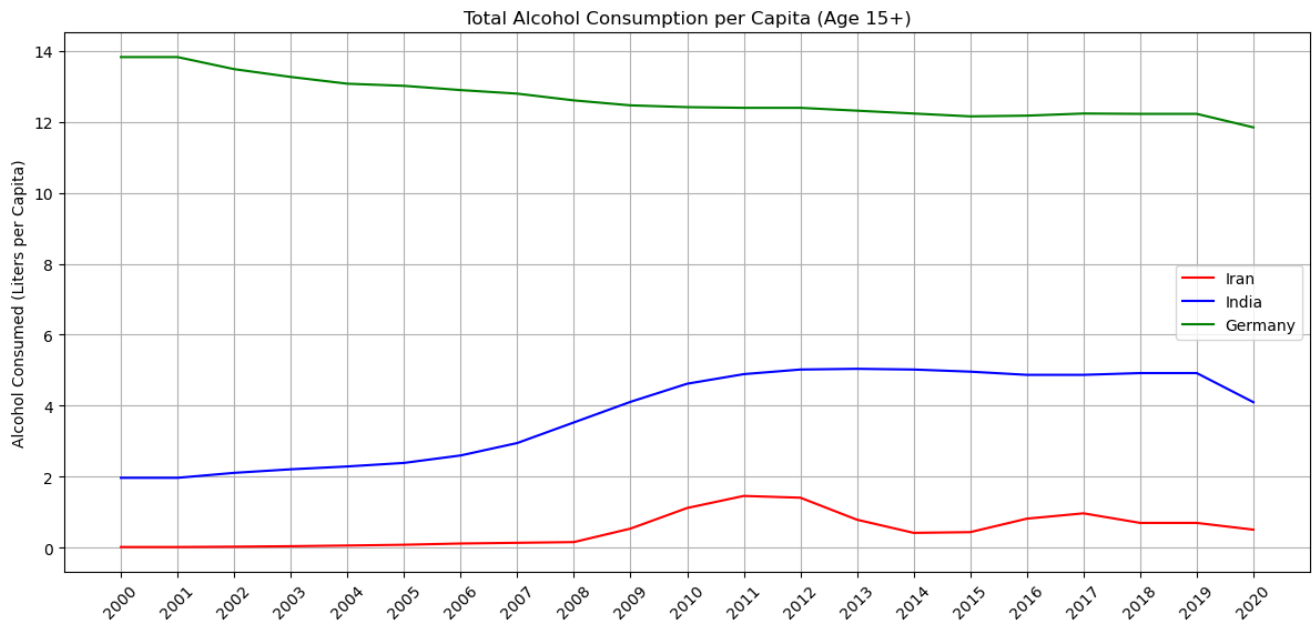
\includegraphics[width=0.8\textwidth]{figure-1.png}
		\caption{Annual per-capita alcohol consumption (2000--2020).}
		\label{fig:trend}
	\end{figure}
	
	\subsection{Distributional Comparisons}
	Table~\ref{tab:stats} summarizes empirical statistics. Iran exhibits strong right skew (skewness~$=+1.8$), India left skew (skewness~$=-0.7$), and Germany slight right skew (skewness~$=+0.5$). Kolmogorov--Smirnov tests confirm significant differences between each pair (all $p<0.01$).
	
	\begin{table}[ht]
		\centering
		\caption{Descriptive statistics of per-capita alcohol consumption (2000--2020).}
		\label{tab:stats}
		\begin{tabular}{lccccccc}
			\toprule
			Country & Mean & Median & Mode & IQR & Min & Max & Skewness \\
			\midrule
			Iran    & 0.50  & 0.44   & 0.02 & 0.70 & 0.02 & 1.46 & +1.8 \\
			India   & 3.78  & 4.11   & 1.97 & 2.53 & 1.97 & 5.04 & $-0.7$ \\
			Germany & 12.66 & 12.41  & 12.22& 0.78 &11.84 &13.82 & +0.5 \\
			\bottomrule
		\end{tabular}
	\end{table}
	
	\subsection{Visual Distributional Comparisons}
	
	\begin{figure}[ht]
		\centering
		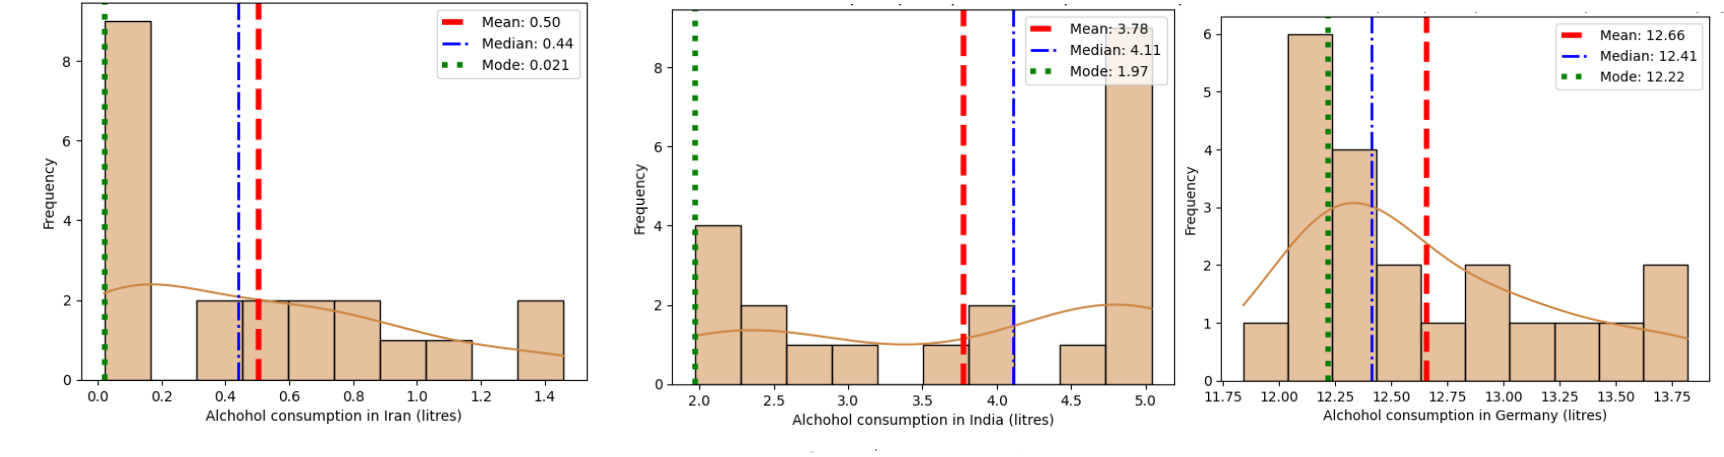
\includegraphics[width=0.8\textwidth]{figure-2.png}
		\caption{Histograms and KDE plots for alcohol consumption by country.}
		\label{fig:hist-kde}
	\end{figure}
	
	\begin{figure}[ht]
		\centering
		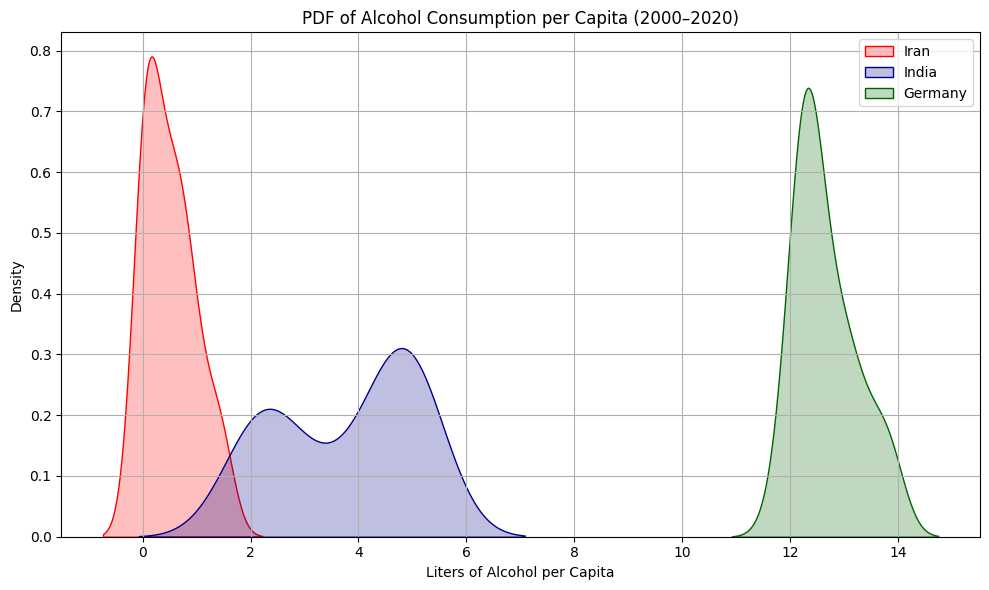
\includegraphics[width=0.8\textwidth]{figure-3.png}
		\caption{Empirical cumulative distribution functions (ECDFs).}
		\label{fig:ecdf}
	\end{figure}
	
	\begin{figure}[ht]
		\centering
		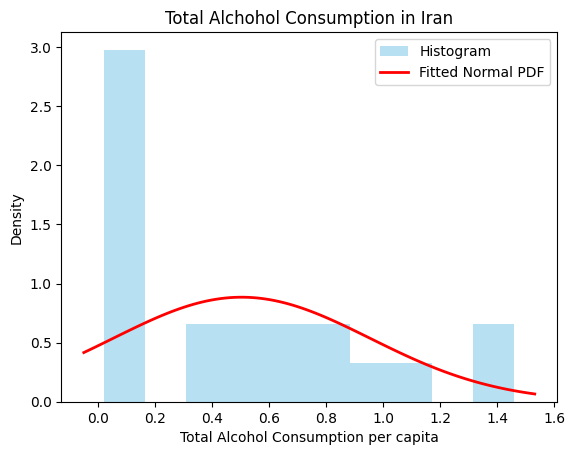
\includegraphics[width=0.48\textwidth]{figure-4a.png}
		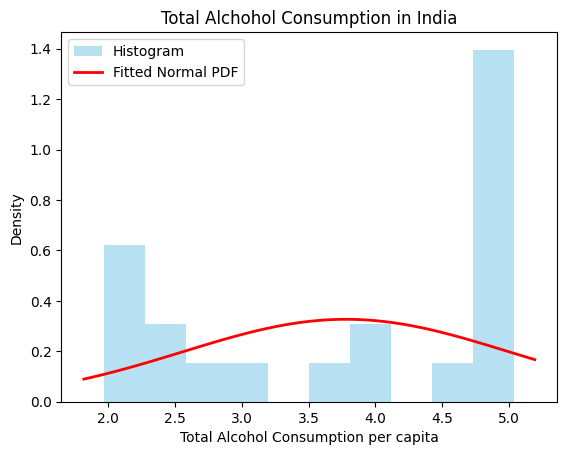
\includegraphics[width=0.48\textwidth]{figure-4b.png}
		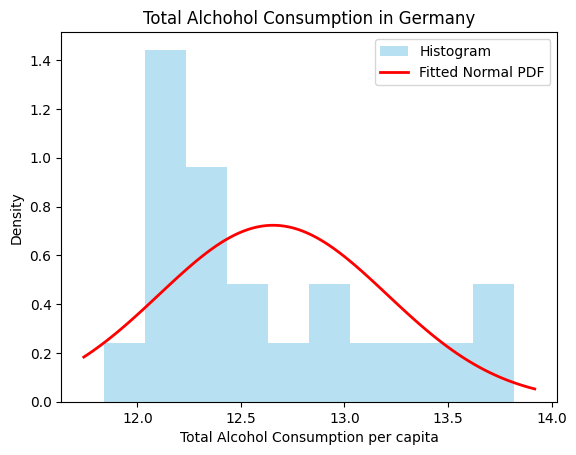
\includegraphics[width=0.48\textwidth]{figure-4c.png}
		\caption{Q--Q plots for Iran (a), India (b), and Germany (c).}
		\label{fig:qqplots}
	\end{figure}
	
	\subsection{Parametric Fitting and Normality}
	Shapiro--Wilk tests (Table~\ref{tab:sw}) reject normality for Iran and India ($p<0.01$) and marginally for Germany ($p=0.04$).
	
	\begin{table}[ht]
		\centering
		\caption{Shapiro--Wilk normality test results.}
		\label{tab:sw}
		\begin{tabular}{lcc}
			\toprule
			Country & $p$-value & Conclusion \\
			\midrule
			Iran    & $<0.01$  & Reject normality \\
			India   & $<0.01$  & Reject normality \\
			Germany & $0.04$   & Marginally non-normal \\
			\bottomrule
		\end{tabular}
	\end{table}
	
	\begin{figure}[ht]
		\centering
		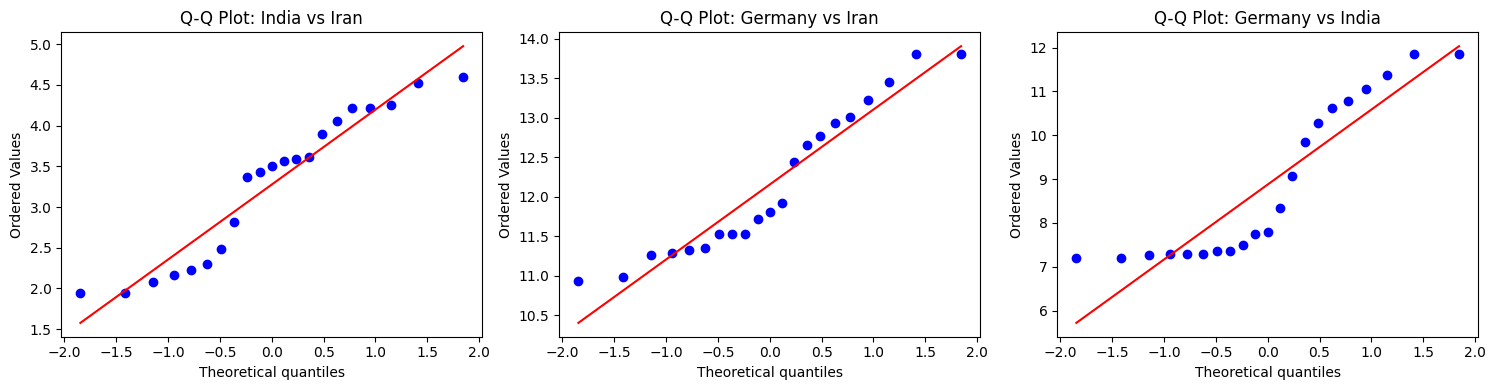
\includegraphics[width=0.8\textwidth]{figure-5.png}
		\caption{Shapiro--Wilk test statistics for each country.}
		\label{fig:sw}
	\end{figure}
	
	\subsection{Trend Tests}
	Mann--Kendall tests (Figure~\ref{fig:mk}) indicate significant increasing trends in Iran ($p=0.00016$) and India ($p=0.00003$), and a significant decreasing trend in Germany ($p<10^{-8}$).
	
	\begin{figure}[ht]
		\centering
		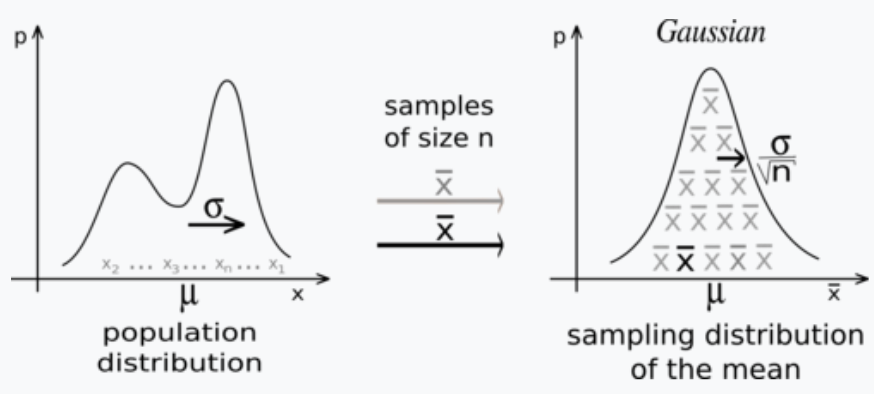
\includegraphics[width=0.8\textwidth]{figure-6.png}
		\caption{Mann--Kendall trend test results.}
		\label{fig:mk}
	\end{figure}
	
	\subsection{Bootstrap and Central Limit Theorem}
	Bootstrap resampling yields distributions approximating normality for India and Germany but remaining non-normal for Iran.
	
	\begin{figure}[ht]
		\centering
		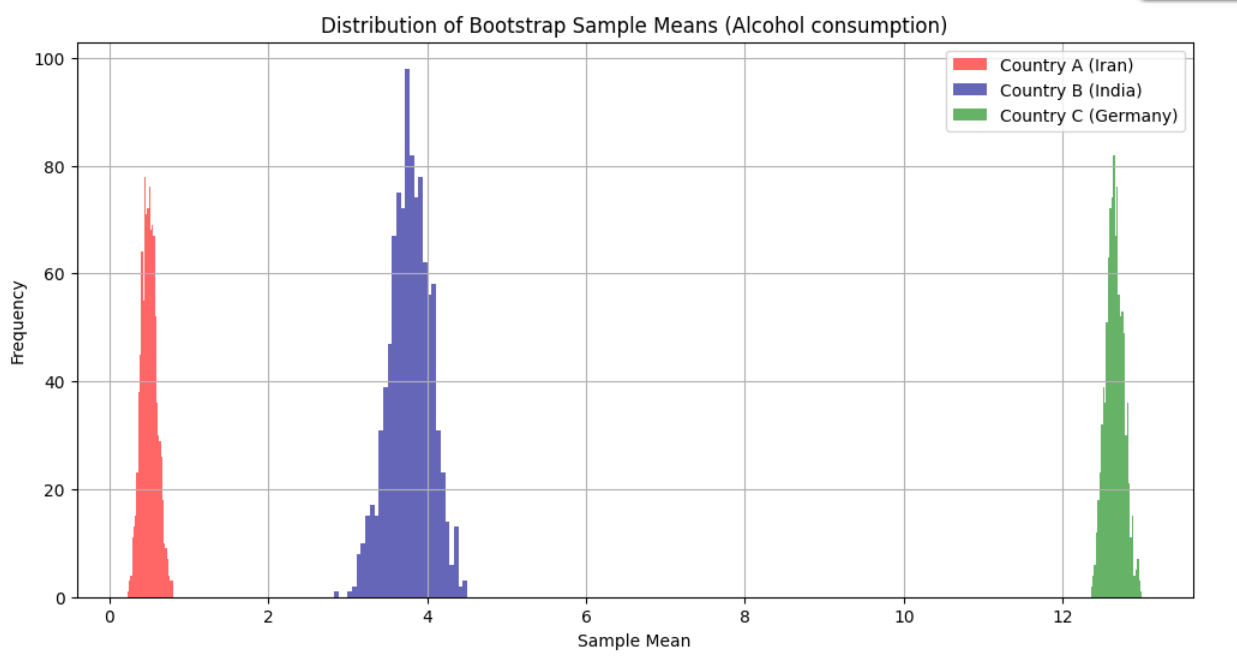
\includegraphics[width=0.8\textwidth]{figure-7.png}
		\caption{Bootstrap distributions of sample means.}
		\label{fig:bootstrap-dist}
	\end{figure}
	
	\begin{figure}[ht]
		\centering
		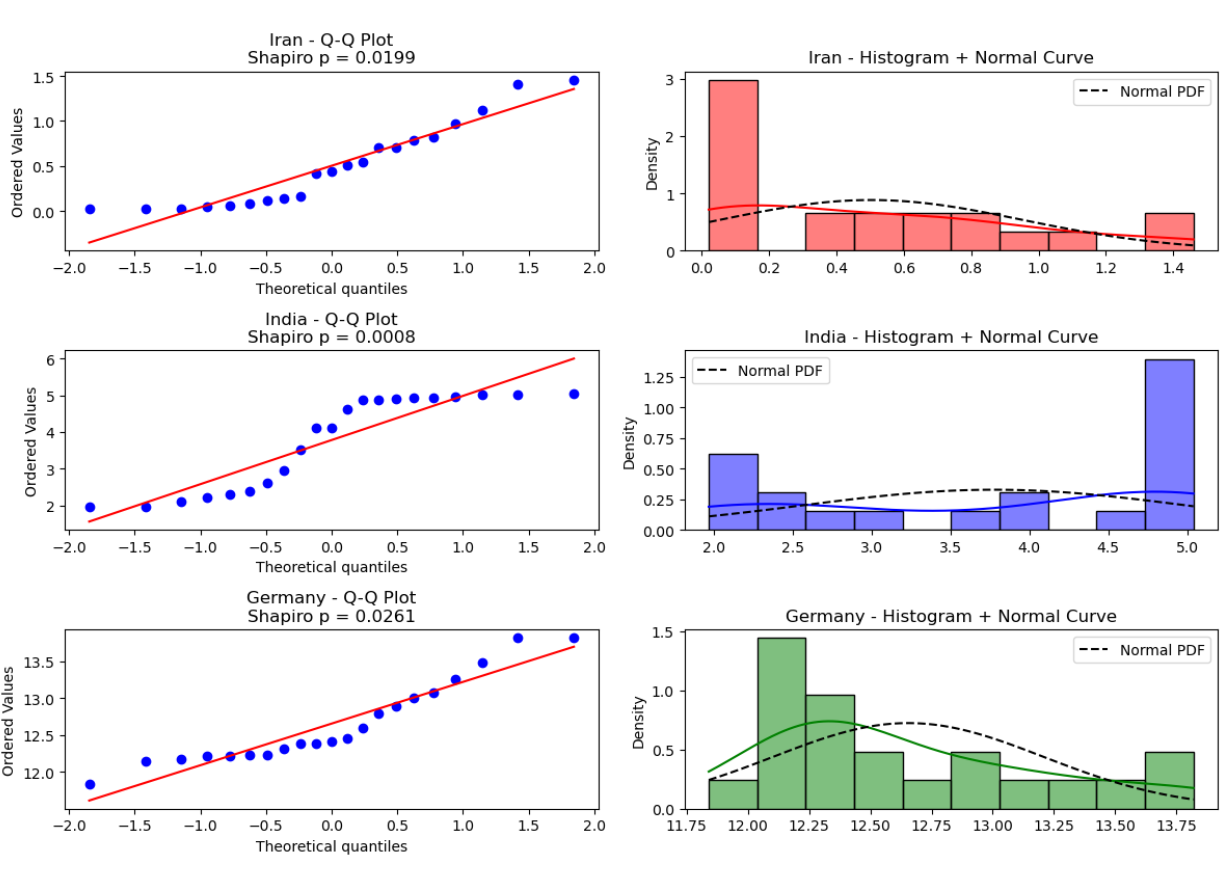
\includegraphics[width=0.8\textwidth]{figure-8.png}
		\caption{Normality test results on bootstrap means.}
		\label{fig:bootstrap-normality}
	\end{figure}
	
	\section{Conclusion}
	This study elucidates distinct consumption patterns in three countries, with Germany exhibiting high but declining use, India rising then moderately declining, and Iran consistently low. Distributional analyses and normality tests highlight non-normality in original series. Bootstrap results affirm the Central Limit Theorem for moderate-to-large variability series (India, Germany) but caution in small, skewed samples (Iran). These findings demonstrate the utility of combined descriptive, inferential, and resampling methods in public-health data analysis.
	
	\section*{References}
	\begin{enumerate}
		\item World Bank (2025). World Development Indicators: Alcohol consumption, total (liters of pure alcohol, age 15+). Retrieved May 1, 2025, from \url{https://databank.worldbank.org/}
		\item Wikipedia (2024). Central Limit Theorem. Retrieved April 29, 2024, from \url{https://en.wikipedia.org/wiki/Central_limit_theorem}
		\item OpenAI (2025). ChatGPT response to "refer ChatGPT in Chicago format". Retrieved May 1, 2025, from \url{https://chat.openai.com/}
	\end{enumerate}
	
\end{document}
